
\chapter{Hashes}
\label{hashes}

Este capítulo presenta otro tipo integrado conocido como un
hash. Los hashes son unas de las mejores y más comunes 
características de Perl; ellos constituyen los componentes básicos
de muchos algoritmos eficientes y elegantes.

\section{Un Hash es un Mapeo}
\label{hash_descr}

\index{hash}
\index{type!hash}
\index{key}
\index{key-value pair}
\index{index}
\index{mapping}
Un {\bf hash} es como un array, pero más general. En un array,
los índices o subíndices tienen que ser enteros; en un hash,
pueden ser (casi) cualquier cosa.

Un hash contiene una colección de índices, los cuales se llaman
{\bf claves}, y una colección de valores. 
Cada llave está asociada a un valor único. Una clave y un valor
juntos forman un par (un objeto del tipo Pair), o un {\bf par
clave-valor}. Un hash puede ser visto como una colección de parejas de
clave-valor. Los valores en un hash puede también llamarse artículos o 
elementos, como con los arrays.
\index{item}

En otros lenguajes de programación, los hashes son algunas veces
llamados diccionarios, tablas hash, mapas, o arrays asociativos.

En el lenguaje matemático, un hash representa a un {\bf mapeo}
desde las claves a los valores, así que puedes también decir que cada
clave ``mapea`` a un valor. Como un ejemplo, construiremos un hash
que mapea palabras del inglés al español, y por lo tanto las llaves y
los valores son todos cadenas de texto.

En Perl, el nombre de un hash comienza con el sigilo ``\verb|%|``. Para
crear un nuevo hash, solo decláralo de esta manera:
\index{sigil}
\index{sigil, percent}

\begin{lstlisting}
> my %ingAesp;
\end{lstlisting}

Esto crea un hash vacío. Para agregar artículos al hash,
puedes usar llaves:
\index{curly bracket}
\index{bracket!curly}
\index{brace}

\begin{lstlisting}
> %ingAesp{'one'} = 'uno';
uno
\end{lstlisting}
%
Esta línea crea un artículo que relaciona la clave
\verb"'one'" al valor \verb"'uno'".  

Si la clave es una cadena de texto que contiene una sola palabra
(i.e., sin ningún espacio en el medio), existe un atajo más 
idiomático para crear la misma entrada de hash:
\index{idiomatic}

\begin{lstlisting}
> %ingAesp<one> = 'uno';
uno
\end{lstlisting}
%
Si imprimimos el hash, vemos un par clave-valor con el 
operador constructor de pares \verb|=>| entre la clave y
el valor:
\index{pair constructor}

\begin{lstlisting}
> say %ingAesp;
one => uno
\end{lstlisting}
%
Este formato de salida es también un formato de entrada.
Por ejemplo, puedes crear un hash nuevo con tres artículos:

\begin{lstlisting}
> my %ingAesp = ('one' => 'uno', 'two' => 'dos', 'three' => 'tres');
one => uno, three => tres, two => dos
\end{lstlisting}
%

El uso del operador constructor de pares \verb|=>| entre claves y 
valores no es requerido; puedes usar comas tambíen:

\begin{lstlisting}
my %ingAesp = ('one', 'uno', 'two', 'dos', 'three', 'tres');
\end{lstlisting}
%

Pero el constructor de pares tiene la ventaja de mostrar
gráficamente las relaciones clave-valor. El operador constructor
de pares también hace que el uso de comillas no mandatario
en su lado izquierdo (provisto que la clave sea una cuerda 
de texto sin espacios):

\begin{lstlisting}
> my %ingAesp = (one => 'uno', two => 'dos', three => 'tres');
one => uno, three => tres, two => dos
\end{lstlisting}
%

También podrías usar una sintaxis de lista más concisa para la
asignación del hash y Perl convertirá felizmente la lista
en un hash, provisto que el número de artículos en la lista 
de entrada sea par:

\begin{lstlisting}
> my %ingAesp = <one uno two dos three tres>;
one => uno, three => tres, two => dos
\end{lstlisting}
%

Podrías sorprenderte con el resultado. El orden de los
pares clave-valor usualmente no se encuentran en el orden
en el cual lo poblaste. En general, el orden de los artículos
en un hash es impredecible.

Pero eso no es un problema porque los elementos de un hash
nunca son indexados con subíndices enteros. En lugar de esto,
usas las claves para consultar los valores correspondientes:

\begin{lstlisting}
> say %ingAesp<two>;
dos
\end{lstlisting}
%
La clave \verb"two" siempre mapea al valor \verb|`dos`|
así que el orden de los artículos no importa.

Si la clave no se encuentra en el hash, obtienes un valor 
indefinido:

\begin{lstlisting}
> say %ingAesp<four>;
(Any)
\end{lstlisting}
%
El método o la función {\tt elems} funciona con los hashes
como con los array; devuelve el número de pares clave-valor:
\index{elems function or method}
\index{function!elems}
\index{elems function or method}
\index{method!elems}


\begin{lstlisting}
> say %ingAesp.elems;
3
> say elems %ingAesp
3
\end{lstlisting}
%
El adverbio {\tt :exists} también funciona con los hashes 
como con los arrays; te dice si algo aparece como una 
{\em clave} en el hash (aparecer como un valor no es suficiente)
\footnote{Evaluar el valor en un contexto Booleano también 
funcionaría con nuestro ejemplo, pero esto devolvería
algo erróneo cuando la clave existe, pero el valor 
no está definido o por lo contrario evalúa a un valor falso
(por ejemplo, si es igual a {\tt False}, cero, o 
cadena de texto vacía).}:
\index{membership!hash}
\index{exists adverb}
\index{adverb!:exists}

\begin{lstlisting}
> %ingAesp<two> :exists;
True
> %ingAesp<four> :exists;
False
\end{lstlisting}
%
Para chequear si algo aparece como un valor en un hash, 
puedes usar el método {\tt values}, el cual devuelve una 
colección de valores, y después usar un bucle (o posiblemente 
{\tt grep}) para buscar el artículo:
\index{values function or method}
\index{method!values}
\index{grep}

\begin{lstlisting}
my @vals = values %ingAesp;
for @vals -> $value {
    say "!`Encontrado!" if $value eq 'uno';           # -> !`Encontrado!
}
\end{lstlisting}
%
O más concisamente:
\begin{lstlisting}
say "!`Encontrado!" if grep {$_ eq 'uno'}, %ingAesp.values;
\end{lstlisting}

Dado que {\tt grep}  usa por defecto una coincidencia inteligente, 
esto puede hacerse de una forma aún más concisa:

\begin{lstlisting}
say "!`Encontrado!" if grep {'uno'}, %ingAesp.values;  # -> !`Encontrado!
\end{lstlisting}

Cuando se inspecciona los valores, el programa tiene que buscar 
los elementos de la lista en orden (o en secuencia), como en la
Sección~\ref{find}. A medida que la lista se vuelve más larga, 
el tiempo de búsqueda se extiende en proporción directa.
\index{sequential search}
\index{search!sequential}

Por el contrario, cuando se inspecciona las claves, Perl usa
un algoritmo de {\bf hashing} que tiene una propiedad interesante:
toma el mismo monto de tiempo sin importar cuantos artículos
se encuentren en el hash. En otras palabras, funciona bastante 
rápido, comparado con el tamaño de la lista, cuando la lista
que se inspecciona es larga. Ésta es la razón por la cual la
solución al ejercicio de par reverso (Ejercicio~\ref{reverse_pair})
del capítulo anterior usando un hash fue casi tres veces más rápido
que la solución de búsqueda binaria (ver Subsección~\ref{sol_reverse_pair}).

\label{ex_employees}
Como ejercicio, usa la muestra de los datos de empleados del 
array multidimensional  de la Sección~\ref{multidimensional_array}
(p.~\pageref{multidimensional_array}), organízala en un hash, y 
busca algunos salarios. Pista: no necesitas una estructura 
multidimensional para hacer eso con un hash.
Solución: \ref{sol_ex_employees}


\section{Operaciones Comunes con Hashes}

Ya vimos que para poblar un hash, puedes asignarle una lista 
par. Las cuatros formas sintácticas siguientes son correctas:

\begin{lstlisting}
my %primer_trimestre  = ("ene" => 1, "feb" => 2, "mar" => 3);
my %segundo_trimestre = (abr => 4, may => 5, jun => 6);
my %tercer_trimestre  = jul => 7, aug => 8, sep => 9;
my %cuarto_trimestre  = < oct 10 nov 11 dec 12 >;
\end{lstlisting}

Para agregar un elemento a un hash, solo asigna el hash con
una clave:

\begin{lstlisting}
my %meses = ("ene" => 1, "feb" => 2, "mar" => 3);
%meses{'abr'} = 4;
say %meses;         # -> abr => 4, feb => 2, ene => 1, mar => 3
\end{lstlisting}

Recuerda que también puedes hacer lo mismo sin encerrar 
las claves en comillas si usas el operador quote-word con
las comillas angulares (si las claves son cadenas de texto):
\index{quote-word operator}
\index{angle bracket}

\begin{lstlisting}
%months<abr> = 4;       # igual que: %meses{'abr'} = 4;
\end{lstlisting}

o puedes usar la función {\tt push} con un par:
\index{push function}
\index{function!push}

\begin{lstlisting}
> push %meses, (may => 5);
abr => 4, feb => 2, jan => 1, mar => 3, may => 5
> my $nuevo-par = jun => 6
jun => 6
> push %meses, $nuevo-par;
abr => 4, feb => 2, jan => 1, jun => 6, mar => 3, may => 5
\end{lstlisting}
%

Usar {\tt push} para agregar un par a un hash no es exactamente lo
mismo que hacer una asignación de hash: si la clave ya existe,
el valor antiguo no es reemplazado por el valor nuevo---en lugar,
ambos valores son colocados en un array (o si el valor antiguo se 
encuentra ya en el array, entonces el valor nuevo se agrega al 
array):

\begin{lstlisting}
> push %meses, (jan => '01');
{abr => 4, feb => 2, jan => [1 01], jun => 6, mar => 3, may => 5}
\end{lstlisting}

Para chequear si un valor está definido para una clave dada,
usa {\tt defined}:
\index{defined}

\begin{lstlisting}
> say True if defined %meses<abr>;
True
\end{lstlisting}
%

Para obtener el número de artículos en un hash, usa el 
método {\tt elems}:
\index{elems function or method}

\begin{lstlisting}
say %meses.elems;                # -> 6
\end{lstlisting}

Para remover un artículo del hash, usa el adverbio {\tt :delete}:
\index{delete adverb}
\index{adverb!:delete}

\begin{lstlisting}
> push %meses, (jud => 7);      # !`Oops, un error!
abr => 4, feb => 2, jan => 1, jud => 7, jun => 6, mar => 3, may => 5
> %meses{'jud'}:delete;         # error removido
7
> say %meses
abr => 4, feb => 2, jan => 1, jun => 6, mar => 3, may => 5
\end{lstlisting}

Nota que el adverbio {\tt :delete} también devuelve le valor que
ha sido removido.

Para interar sobre un hash, usa:
To iterate over a hash, use:
\index{kv function or method}
\index{keys function or method}
\index{values function or method}
\index{pairs function or method}

\begin{itemize}
\item {\tt kv} para extraer las claves y los valores intercalados;
\item {\tt keys} para extraer las llaves;
\item {\tt values} para extraer los valores;
\item {\tt pairs} para extraer los pares clave-valor;
\end{itemize}

Por ejemplo:

\begin{lstlisting}
> for %meses.kv -> $clave, $val { say "$clave => $val" }
jan => 1
abr => 4
mar => 3
jun => 6
may => 5
feb => 2
> say keys %meses;
(jan abr mar jun may feb)
> say values %meses;
(1 4 3 6 5 2)
> say %meses.pairs;
(jan => 1 abr => 4 mar => 3 jun => 6 may => 5 feb => 2)
\end{lstlisting}
%

\section{Un Hash como una Colección de Contadores}
\label{histogram}
\index{counter}

Supón que se te provee con una cadena de texto y quieres contar
el número de apariciones de cada letra. Existen varias maneras
en las que puedes hacer esto:

\begin{itemize}

\item Podrías crear 26 variables, una por cada letra del 
alfabeto. Después podrías travesar la cadena de texto y, por cada
carácter, aumentar el contador correspondiente, probablemente
usando una condicional encadenada grande y fea de 26 partes.

\item Podrías crear un array con 26 elementos. Después podría
convertir cada carácter a un número (usando la función integrada
{\tt ord}), usar el número como un índice en el array, e 
incrementar el contador apropiado.

\item Podrías crear un hash con caracteres como claves y contadores
como los valores correspondientes. La primera vez que ves un carácter,
agregarías un artículo al hash. Después de eso, aumentarías el valor
de un artículo existente.
\end{itemize}

Cada una de estas opciones realiza la misma computación,
pero cada una de ellas implementa la computación en una
manera distinta.
\index{implementation}

Una {\bf implementación} es una manera de realizar una computación;
algunas implementaciones son mejores que otras. Por ejemplo,
una ventaja de la implementación con el hash es que no tenemos
que saber con antelación cuales letras aparecen en la 
cadena de texto y solo tenemos que crear espacio para las letras
que si aparecen.

Aquí se muestra como el código podría lucir:

\begin{lstlisting}
sub histograma (Str $cadena) {
    my %histo;
    for $cadena.comb -> $letra {
        %histo{$letra}++;
    }
    return %histo;
}
\end{lstlisting}
%
El nombre de la función es {\tt histograma}, el cual es
un término estadístico para una colección de contadores (o frecuencias).
\index{histogram}
\index{frequency}
\index{traversal}
\index{comb function and method}
\index{counter}

La primera línea de la función crea un hash vacío.
El bucle {\tt for} traversa la cadena. Cada vez a través
del bucle, si el carácter \verb|$letra| no está en el hash, Perl
crea un artículo nuevo con la clave \verb|$letra| y fija los 
valores 0 cuando el operador ++, así que el primer valor 
inmediatamente después de eso es 1. Si la \verb|$letra| 
ya se encuentra en el hash, el valor se incrementa.
\index{increment operator}

Así es cómo funciona:

\begin{lstlisting}
> say histograma("We all live in a yellow submarine")
W => 1, a => 3, b => 1, e => 4, i => 3, l => 5, (...) y => 1
\end{lstlisting}
%
El histograma indica que las letras \verb|`W`| y \verb|`b`|
aparecen solo una vez; \verb|`a`| y \verb|`i`| aparecen
tres veces, \verb|`e`| aparece cuatro veces, etc.

\section{Bucles y Hashes}
\index{hash!looping with}
\index{looping!with hashes}
\index{traversal}

Si usas un hash en una sentencia {\tt for}, el bucle 
traversa los pares del hash:

\begin{lstlisting}
> for %ingAesp -> $par { say $par}
two => dos
three => tres
one => uno
\end{lstlisting}
%

Hemos nombrado la variable de iteración \verb|$par| para
resaltar más claramente que el programa está iterando
sobre los pares clave-valor (actualmente objetos \verb|Pair|).
Puedes usar los métodos {\tt key} y {\tt value} (nota que
están en singular) para acceder
la clave y valor de un \verb|Pair|. Por ejemplo, para revertir
el orden en el cual cada línea es imprimida:

\begin{lstlisting}
> for %ingAesp -> $par { say $par.value ~ " <= " ~ $par.key; }
dos <= two
tres <= three
uno <= one
\end{lstlisting}

Otra vez, las claves no estás en un orden particular. Para
travesar las claves ordenadamente, puedes usar las funciones
o métodos {\tt keys} (en plural) y {\tt sort}:
\index{keys function or method}
\index{method!keys}
\index{sort!function or method}
\index{method!sort}

\begin{lstlisting}
my %histo = histograma("We all live in a yellow submarine");
for %histo.keys.sort -> $clave {
    say "$clave\t%histo{$clave}";
}
\end{lstlisting}



\section{Búsqueda Inversa}
\label{raise}
\index{hash!lookup}
\index{hash!reverse lookup}
\index{lookup, hash}
\index{reverse lookup, hash}

Dado un hash \verb|%hash| y una clave \verb|$k|, es fácil 
encontrar el valor correspondiente \verb|$val = %hash{$k}|.
Esta operación se conoce como una {\bf búsqueda} y, como ya
mencionamos, esta es bastante rápida hasta cuando el hash
es bien grande.
\index{lookup}
\index{hash lookup}

?`Qué pasa si tienes a \verb|$val| y quieres encontrar a \verb|$k|?
Sucede que tienes tres problemas: primero, podrían existir más
de una clave que mapean al valor \verb|$val|; dependiendo de
la aplicación, podrías elegir una, o tendrías que crear un array 
que las contenga a todas. Segundo, no existe una sintaxis simple
para hacer una {\bf búsqueda inversa}; tienes que hacer la búsqueda.
Tercero, podría consumir mucho tiempo si el hash es largo.

Aquí presentamos una función que toman un valor y devuelve
la primera clave que mapea a ese valor:
\index{reverse lookup}

\begin{lstlisting}
sub busqueda-inversa (%hash, $val) { 
    for %hash -> $par { 
        return $par.key if $par.value eq $val;
    }
    return;
}
\end{lstlisting}
%
Esta subrutina es otro ejemplo del patrón de búsqueda. 
Si llegamos al final del bucle, eso significa que \verb|$val|
no aparece en el hash como un valor, así que devolvemos un 
valor indefinido (Nil). Aquí, la responsabilidad para reaccionar
a tal situación se deja a la función que hace la llamada. 
Una alternativa es levantar una excepción, la cual tendría
que ser todavía la responsabilidad de la función que hace la
llamada. Sin embargo, dado que la búsqueda directa con la clave
no levanta una excepción pero simplemente devuelve un valor indefinido
cuando la clave no existe, hace sentido que {\tt busqueda-inversa}
tenga el mismo comportamiento cuando el valor no se encuentra.

Este es un ejemplo de una búsqueda inversa exitosa:

\begin{lstlisting}
> my %histo = histograma('parrot');
a => 1, o => 1, p => 1, r => 2, t => 1
> my $clave =  busqueda-inversa %histo, "2";
r
\end{lstlisting}
%
Y una búsqueda sin éxito:

\begin{lstlisting}
> say busqueda-inversa %histo, "3";
Nil
\end{lstlisting}
%

Otra forma más concisa de hacer la búsqueda inversa sería
usar {\tt grep} para extraer una lista de valores 
que satisfagan nuestra condición:
\begin{lstlisting}
say grep { .value == 2 }, %histo.pairs;   # -> (r => 2)
\end{lstlisting}

Otra opción es usar una expresión con la función integrada
{\tt first} para extraer solo el primer para:
\begin{lstlisting}
my %histo = histograma('parrot');
say %histo.pairs.first: *.value == 1;      # ->  p => 1
\end{lstlisting}

\index{whatever}
Este último ejemplo usa el parámetro \emph{whatever} ``*``
el cual no hemos discutido en este libro todavía. Digamos que,
aquí, el ``*`` quiere decir sucesivamente para cada par del hash
y la función {\tt first} devuelve el primer par que coincide
con la condición del valor (ver 
Sección~\ref{whatever star parameter} para detalles sobre
el parámetro ``*``).

Una búsqueda inversa es mucha más lenta que una búsqueda directa;
si tienes que hacerla constantemente, o si el hash se vuelve grande,
el rendimiento de tu programa sufrirá.
\index{reverse lookup}

\section{Comprobando la Existencia}
\index{existence!testing for}

Una tarea bastante común es determinar sin algo existe o si un valor
dado ya se ha visto en un programa. El uso de un hash es usualmente
la mejor solución porque encontrar si existe una entrada para un valor
dado es muy simple y también muy eficiente: solo necesitas almacenar los
valores que quieres inspeccionar como una entrada de clave, y después 
chequear por su existencia cuando sea necesario.

En tal caso, usualmente el valor no es importante y podrías
colocar cualquier cosa. Es muy común en este caso usar ``1`` como
un valor, pero también podrías almacenar {\tt True} o cualquier
otro valor que desees.

Supón que queremos generar 10 números enteros aleatorios entre 0
y 49, pero queremos asegurarnos que los enteros son únicos. Podemos
usar el método {\tt rand} 10 veces con el rango deseado. Pero la
posibilidad de obtener el mismo número dos veces no es tan
insignificante (ver Ejercicio~\ref{birthdays} sobre la 
paradoja del cumpleaños y su solución (Subsección~\ref{sol_birthdays}) 
para una situación similar). Por ejemplo, al intentar esto:
\index{duplicate!checking}
\index{rand function}

\begin{lstlisting}
> my @lista;
[]
> push @list, 50.rand.Int for 1..10;
> say @lista;
[12 25 47 10 19 20 25 42 33 20]
\end{lstlisting}

se produjo un valor duplicado en la lista (25) en el primer intento.
Y el segundo intento produjo tres pares de duplicados:

\begin{lstlisting}
> say @lista;
[45 29 29 27 12 27 20 5 28 45]
\end{lstlisting}

Podemos usar un hash para rechazar cualquier entero aleatorio
generado que ya se haya visto. La siguiente manera sería una forma
de escribir esto en código:
\index{rand function}

\begin{lstlisting}
my @lista;
my %visto;
while @lista.elems < 10 {
    my $aleatorio = 50.rand.Int;
    next if %visto{$aleatorio}:exists;
    %visto{$aleatorio} = 1;
    push @lista, $aleatorio;
}
say @lista;
\end{lstlisting}

Cada valor entero generado se agrega al hash \verb|%visto| 
y la lista de salida. Pero antes de hacer eso, el entero 
generado se chequea con el hash \verb|%visto| para verificar
que no se ha visto todavía. Cuando el programa finaliza su 
ejecución, la lista contiene 10 enteros únicos y (pseudo)aleatorios.

Lo hicimos paso a paso y mantuvimos dos estructuras de datos 
separadas, el array de salida \verb|@lista| y el hash \verb|%visto|,
para hacer el proceso tan claro como sea posible. Pero si lo piensas,
\verb|@lista| y \verb|%visto| tienen esencialmente el mismo contenido
a cada paso a través del bucle. Realmente no tenemos que mantener un
registro de los mismos datos en dos lugares. Dado que tener un hash
es importante para chequear que los valores de salida son únicos, 
podemos deshacernos de \verb|@lista| y escribir una versión más
concisa y probablemente más idiomática del mismo programa:
\index{idiomatic}
\index{push function}

\begin{lstlisting}
my %visto;
while %visto.elems < 10 {
	my $aleatorio = 50.rand.Int;
	push %visto, ($aleatorio => 1) unless %visto{$aleatorio}:exists;
}
say keys %visto;      # -> (39 12 46 27 14 21 4 38 25 47)
\end{lstlisting}

Esto puede simplificarse aún más. No es realmente necesario
chequear si el entero generado existe en el hash: si existe,
el elemento antiguo del hash será reemplazado con el nuevo, 
y el hash esencialmente no cambiará. Además, cuando se evalúa
en un contexto numérico escalar, un hash devuelve el número de
sus elementos, así que la invocación {\tt .elems} no es necesaria.
Esta es la nueva versión:
\index{scalar context}
\index{elems function or method}

\begin{lstlisting}
my %visto;
%visto{50.rand.Int} = 1 while %visto < 10;
say keys %visto;      # -> (46 19 5 36 33 1 20 45 47 30)
\end{lstlisting}

Esta última versión es probable más concisa y más idiomática,
pero esto significa que es mejor. Es perfectamente aceptable
si prefieres la segunda o la primera versión porque la encuentras
más clara. Usa la versión que desees, o tu propia versión modificada
provisto que realice la tarea prevista. Esto es Perl, \emph{
hay más de una forma para hacer algo} (TIMTOWTDI).
\index{TIMTOWTDI}

% Hay más de una forma para hacer algo (HMDUFPHA)

Sin embargo, nota que la versión pura de hash no mantiene el orden
en el cual los números son generados, así que (pseudo)aleatoriedad
podría no ser tan buena.

También nota que Perl tiene una función o método {\tt pick}
para elegir elementos de forma aleatorio de una lista sin 
repetición.
\index{pick function or method}


\section{Las Claves de un Hash son Únicas}

No es posible tener la misma clave en un hash más de una vez.
El intento de mapear un nuevo valor a una clave reemplazará el
valor antiguo con el nuevo. Aquí presentamos un ejemplo de la
creación de un hash con claves duplicadas:
\index{duplicate}

\begin{lstlisting}
> my %amigos = (Gabo => 5, Miguel => 6, Salomé => 5, Gabo => 7, Jorge => 3)
Miguel => 6, Jorge => 3, Salomé => 5, Gabo => 7
\end{lstlisting}

Dado que dos de nuestros amigos se llaman ``Gabo``,  perdemos los
datos asociados con el primero. Esto es algo con lo cual deberías
cuidadoso: las claves de un hash son únicas, así que perderás algunos
artículos si los datos asociados con tus claves tienen duplicados. 
La siguiente sección mostrará algunas maneras de tratar este posible 
problema.

Pero esta propiedad sobre la singularidad de una clave tiene muchos
aspectos positivos. Por ejemplo, una manera típica de remover los duplicados
de una lista de artículos es asignar los artículos de una lista a las
claves de un hash (el valor no importa); al final del proceso, 
la lista de claves no contiene duplicados:

\begin{lstlisting}
> my @array = < a b c d s a z a r e s d z r a >
[a b c d s a z a r e s d z r a]
> my %único = map { $_ => 1 }, @array;
a => 1, b => 1, c => 1, d => 1, e => 1, r => 1, s => 1, z => 1
> my @array_único = keys %único;
[z a e s d c b r]
\end{lstlisting}

Como puedes ver, los duplicados han sido removidos del 
array de salida. En ejemplos simples como este, la función
integrada {\tt unique} habría sido suficiente para remover los
duplicados de \verb|@array|, pero dentro de un programa más
complejo, es bien común usar un hash (usualmente llamado \verb|%visto|)
para chequear si un valor ya se ha visto.
\index{unique function}
\index{map}

\section{Hashes y Arrays}
\label{invert}

\index{inverting a hash}
\index{hash!invert}
Invertir un hash puede ser muy fácil si se conoce que los valores 
ocurren solamente una sola vez (es decir, son únicos). Considera por ejemplo
un hash que mapea los meses a sus números en el año
(limitamos el ejemplo a cinco ejemplos por brevedad):

\begin{lstlisting}
> my %meses = ene => 1, feb => 2, mar => 3, abr => 4, may => 5;
abr => 4, feb => 2, ene => 1, mar => 3, may => 5
\end{lstlisting}
%

Podemos transformar los pares clave-valor en un lista plana,
invertir la lista, y asignar la lista inversa a un nuevo hash:

\begin{lstlisting}
> my %meses_inv = %meses.kv.reverse;
1 => ene, 2 => feb, 3 => mar, 4 => abr, 5 => may
\end{lstlisting}
\index{kv function or method}
\index{reverse function or method}
%

Ahora tenemos un nuevo hash que mapea los números de los meses
a sus nombres. Esto puede ser útil si se conoce que un hash es biyectivo,
pero esta estrategia no funciona correctamente si un valor aparece más de una
vez: en tal caso, algunos pares se perderán:

\begin{lstlisting}
> my %meses = ene => 1, enero => 1, febrero => 2, febrero => 2;
feb => 2, febrero => 2, ene => 1, enero => 1
> my %meses_inv = %meses.kv.reverse;
1 => enero, 2 => febrero
\end{lstlisting}

Los arrays pueden aparecer como valores en un hash. Por ejemplo,
su te dan un hash que mapea las letras a las frecuencias, podrías querer
invertirlo; es decir, crear un hash que mapea las frecuencias  a las
letras. Dado que podría haber varias letras con las misma frecuencia, cada
valor en el hash invertido debería ser un array de letras.
\index{inverting a hash}
\index{hash!invert}

La siguiente es una función que invierte un hash similar:

\begin{lstlisting}
sub invertir-hash (%hash-entrada) { 
    my %hash-salida; 
    for %hash-entrada.kv -> $clave, $val {
        push %hash-salida{$val}, $clave; 
    }
    return %hash-salida;
}
\end{lstlisting}
%
Cada paso a través del bucle, un artículo del hash se asigna a las variables
\verb|$clave| y  \verb|$val|, y \verb|$clave| se añade al valor \verb|%hash-salida|
para la clave \verb|$val|; si dicho valor no existe todavía, entonces es creado.
Al final del proceso, los valores de \verb|%hash-salida| son todos arrays anónimos.

Este es un ejemplo:

\begin{lstlisting}
my %rev-hist = invertir-hash histograma 'parrot';
say %rev-hist;
dd %rev-hist;
\end{lstlisting}

Esto mostrará:

\begin{lstlisting}
1 => [p a o t], 2 => [r]
Hash %rev-hist = {"1" => $["p", "a", "o", "t"], "2" => $["r"]}
\end{lstlisting}

Nota que la función {\tt say} provee una representación simple
de los datos del hash, y que la nueva función {\tt dd} (abreviatura 
de ``data dumper`` -- ``vertedero de datos``) usada en este ejemplo
provee información más detallada. {\tt dd} no es comúnmente usada en 
programas normales, pero puede ser útil mientra la depuración de un
programa para mostrar una descripción detallada de una estructura de 
datos compleja.\footnote{Para ser honesto, {\tt dd} no es Perl~6 estándar,
es una característica específica de Rakudo. Una implementación futura de Perl~6 que
no esté basada en Rakudo podría no tenerla.}
\index{say function or method}
\index{dd function}

Por ejemplo, \verb|%hash-salida| contiene dos artículos (dos pares)
cuyos valores son arrays anónimos. Puedes acceder el segundo elemento
del primer array usando el valor del hash \verb|%rev-hist{"1"}|
como si fuera un nombre de array ordinario, con esta simple sintaxis:

\begin{lstlisting}
say %rev-hist{"1"};  # -> a
\end{lstlisting}


\begin{figure}
\centerline
{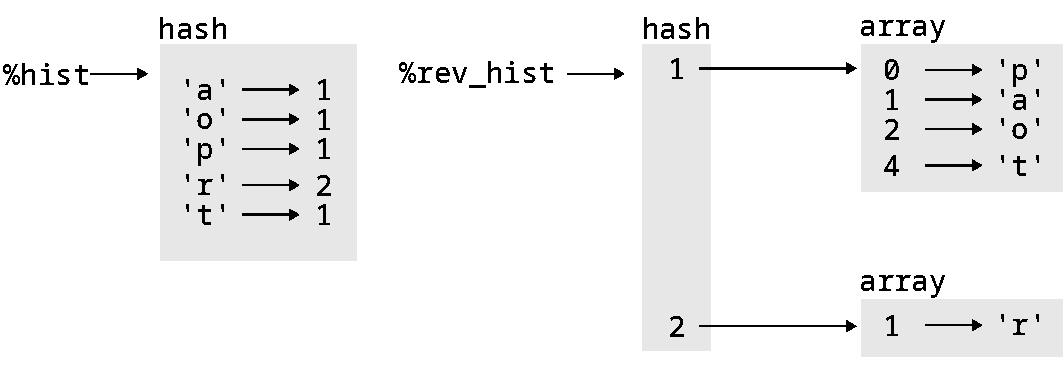
\includegraphics[scale=0.8]{figs/hash1.pdf}}
\caption{Diagrama de estado.}
\label{fig.hash1}
\end{figure}

La figura~\ref{fig.hash1} es un estado de diagrama que muestra a \verb|%hist| 
y a \verb|%rev-hist|. Un hash se representa como una caja con el tipo {\tt hash}
encima y los pares clave-valor dentro.
\index{state diagram}
\index{diagram!state}

Los arrays pueden ser valores en un hash, como este ejemplo muestra, pero
no pueden ser claves. Si intentas hacerlo, probablemente termines con una clave
que contiene solo un elemento del array, pero no lo que esperabas:

\begin{lstlisting}
my @a = 'a' .. 'c';
my %h;
%h{@a} = 5;
say %h;  # -> a => 5, b => (Any), c => (Any)
\end{lstlisting}

Aquí, Perl interpretó la asignación \verb|%h{@a} = 5;|
como una asignación de rebanada, i.e., asumió que intentamos
poblar tres artículos de una vez, una para cada elemento del
array.

\index{hash!function}
\index{hashable}

Como se mencionó anteriormente, un hash se implementa usando 
una función hash y significa que las llaves tienen
que ser {\tt hashable}\footnote{Esto no es del todo verdad.
Las claves de un hash ``normal``deben ser del tipo hashable
y por lo tanto, inmutable. Hay otro tipo de hash, objetos hash,
para los cuales la necesidad de tener claves inmutables no aplica.}.
Una {\bf función hash} es una función que toma un valor (de cualquier tipo)
y devuelve un número entero. Los hashes usan estos enteros, llamados valores
de hash, para almacenar y buscar pares clave-valor.
\index{immutability}

Este sistema funciona bien si las claves son inmutables. Pero si las claves
son mutables, como con los arrays, cosas extrañas pasarían. Por ejemplo,
cuando creas un par clave-valor, Perl aplicaría una función hash a la clave
y la almacenaría en la ubicación correspondiente. Si modificas el clave y después
aplica la función hash nuevamente, entonces sería almacenada en una ubicación
diferente. En ese caso, podrías tener dos entradas para la misma clave, o 
no podría ser capaz de encontrar una clave. En ambos casos, el hash
no funcionaría correctamente.

Esa es la razón por la cual las claves deben ser hashable, y porqué
los tipos mutables como los arrays no lo son. Así que Perl hará algo más 
que puede ser útil (tal como crear tres artículos de hash distintos en el
ejemplo anterior), pero no aplicará la función hash al array. 
  
Dado que los hashes son mutables, ellos no pueden ser usados como claves,
pero {\em pueden} usarse como valores, así que puedes tener hashes anidados.

\section{Memos}
\label{memoize}
\index{memoize}
\index{cache}
\index{memo}
\index{Fibonacci}

Si jugueteaste con la subrutina {\tt fibonacci} en la 
Sección~\ref{one.more.example}, probablemente notaste que 
mientra más grande el argumento, más tiempo toma la subrutina
para ejecutarse. Además, el tiempo de ejecución aumenta extremadamente
rápido.
\index{Fibonacci!function}
\index{function!Fibonacci}

Para entender el porqué, considera la figura~\ref{fig.fibonacci},
la cual muestra la {\bf gráfica de llamada} para {\tt fibonacci} 
con {\tt n=4}.

\begin{figure}
\centerline
{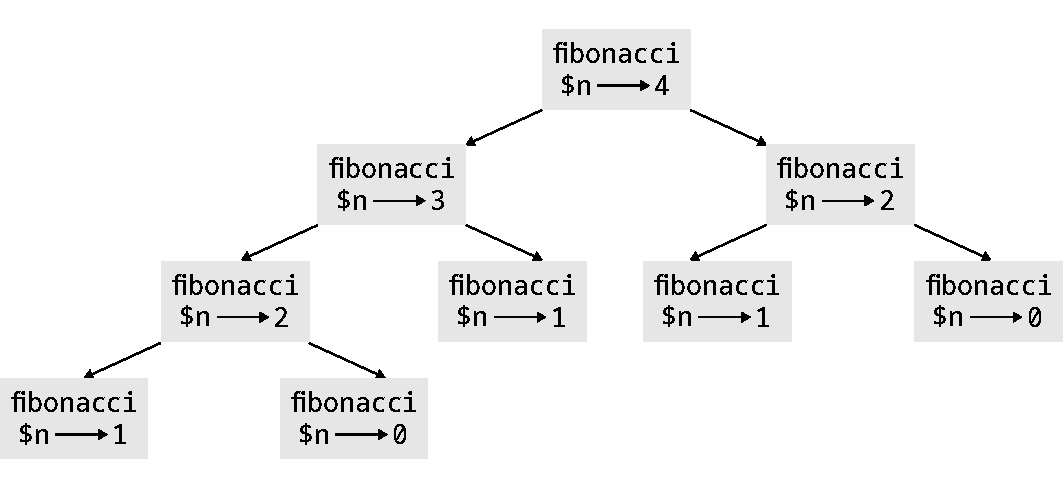
\includegraphics[scale=0.7]{figs/fibonacci.pdf}}
\caption{Gráfica de llamada.}
\label{fig.fibonacci}
\end{figure}

Una gráfica de llamada muestra un conjunto de cuadros de 
una subrutina, con líneas que conectan cada cuadro a los 
cuadros de las funciones que llamas. En la parte superior
de la gráfica, {\tt fibonacci} con \verb|$n=4| llama a \verb|fibonacci|
con \verb|$n=3| y con \verb|$n=2|. En cambio, {\tt fibonacci} con
\verb|$n=3| llama a {\tt fibonacci} con \verb|$n=2| y a \verb|$n=1|,
etcétera.
\index{function frame}
\index{frame}
\index{call graph}

Cuenta cuántas veces {\tt fibonacci(0)} y {\tt fibonacci(1)} 
son llamadas. Esta es una solución ineficiente al problema,
y se vuelve peor a medida que el argumento crece.
\index{memo}

Una solución es mantener un registro de los valores que ya se han
calculado al almacenarlos en un hash. Un valor que se ha computado
y se almacena para uso posterior se conoce como un {\bf memo}. 
Aquí presentamos una versión ``memoizada`` de {\tt fibonacci}:
\index{Fibonacci!memoized}

\begin{lstlisting}
my %conocidos = 0 => 1, 1 => 1;
say fibonacci(10);
sub fibonacci ($n) {
    return %conocidos{$n} if %conocidos{$n}:exists;
    %conocidos{$n} = fibonacci($n-1) + fibonacci($n-2);
    return %conocidos{$n};
}
\end{lstlisting}
%

\verb|%conocidos| es un hash que mantiene un registro
de los números Fibonacci que ya sabemos. Comienza con dos
artículos: 0 y 1, los cuales mapean a 1.

Cuando se llama a {\tt fibonacci}, la subrutina chequea a
\verb|%known|. Si el resultado ya existe, lo devuelve inmediatamente.
De lo contrario, tiene que computar el nuevo valor, 
agregar al hash, y devolverlo.

Si ejecutas esta versión de {\tt fibonacci} y la comparas con
la original, encontrarás que es mucho más rápida, especialmente
para un argumento grande (por ejemplo, mayor que 30).

\index{cache}
\index{memoize}
La memoización es una forma de \emph{caché}, i.e., almacenar en 
memoria el resultado de una computación (presumiblemente costosa)
para evitar computarla nuevamente. Este proceso es algunas veces 
llamado ``negociación de memoria por ciclos de CPU.`` En algunos 
casos, tal como nuestro ejemplo recursivo de Fibonacci, la ganancia
es absolutamente inmensa: calcular el número Fibonacci 100$^{o}$
tomaría billones de años con la subrutina recursiva original
y toma solo segundos con la versión memoizada. 

Nota que en el caso específico de la función Fibonacci,
estamos almacenando valores para cada entero sucesivo; podría
haber memoizado los números Fibonacci en un array en lugar de 
un hash (y podría ser hasta un poco más eficiente), pero usar
un hash para tal propósito es una solución más general, 
lo cual funciona hasta cuando las claves del memo no son
enteros consecutivos.

Como ejercicio, intentar escribir la subrutina {\tt fibonacci}
usando un array en lugar de un hash para memoizar los números
Fibonacci ya calculados.


\section{Hashes como Tablas de Despacho}
\label{dispatch}

Puede necesitar lanzar alguna acción dependiendo en el valor
de un parámetro recibido por el programa. Para hacer eso,
podrías usar una serie de sentencias
\verb'if {...} elsif {...} else {...}' como esta:

\begin{lstlisting}
sub ejecuta-parar   { ... };
sub ejecuta-iniciar { ... };
my $param = obtén-param;
if $param eq "parar" {
    ejecuta-parar;
} elsif $param eq "iniciar" {
    ejecuta-iniciar;
} elsif $param = "a" {
    say $ayuda;
} elsif $param = "ayuda" {
    say $ayuda;
} elsif $param = "v" {
    $verbose = True;
} else {
    die "Opción desconocida $param";
}
\end{lstlisting}

Esta estrategia es aburrida y sujeta a errores. El uso de 
una tabla de despacho es usualmente una solución más simple.

Una tabla de despacho es una estructura de datos que mapea 
identificadores a referencias códigos o objetos de subrutinas.
Si se aplica al escenario anterior, podría lucir así:

\begin{lstlisting}
sub ejecuta-parar   { ... };
sub ejecuta-iniciar { ... };
my %despacho = (
    parar   => &ejecuta-parar,
    iniciar => &ejecuta-iniciar,
    a       => { say $ayuda; },
    ayuda   => { say $ayuda; },
    v       => { $verbose = True;},
);
my $param = obtén-param();
die "Opción desconocida $param" unless %despacho{$param}:exists;
%despacho{$param}(); # ejecuta la acción especificada en %despacho
\end{lstlisting}

El hash \verb|%despacho| define la acción dependiendo en el 
parámetro usado como una clave. La sentencia \verb|%despacho{$param}()|
llama la acción requerida.

Esta estrategia es un poco más concisa y más limpia, pero existen 
otras ventajas. Es más fácil de mantener: si necesitas agregar
una opción, solo necesitas agregar una entrada al hash y evitas
agregar código en el medio de una cadena complicada de sentencias
\verb'if {...} elsif {...} else {...}' lo cual podría estropear algo.

Otra ventaja es que la tabla de despacho puede modificarse
dinámicamente durante el tiempo de ejecución, por ejemplo 
dependiendo en ciertas circunstancias externas (por ejemplo el día
del mes cuando el programa se ejecuta) o de acuerdo a un 
archivo de configuración. Esto significa que es posible 
modificar el comportamiento de un programa dinámicamente 
después del tiempo de compilación, mientras todavía se
ejecuta. Esto abre el camino a algunas técnicas avanzadas de
programación que están fuera del alcance de este libro.

Nota que hemos usado hashes para nuestras tablas de despacho,
y esta es la manera más común de implementarlas. Si hace sentido
tener pequeños enteros como claves, podrías también implementar
una tabla de despacho como un array. Este es el caso, por ejemplo,
los artículos numerados de un menú donde al usuario se le incita
a teclear un número para indicar la opción de menú a activar.


\section{Variables Globales}
\index{global variable}
\index{variable!global}
\index{lexical variable}
\index{variable!lexical}

En el ejemplo anterior sobre Fibonacci memoizado, el hash \verb|%conocidos|
es creado fuera de la subrutina, así que pertenece al 
paquete principal entero. Tales variables con conocidas
como {\bf globales} porque pueden accederse desde cualquier
otra función. A diferencia de variables lexicales ``locales``, 
las cuales desaparecen cuando sus ámbitos terminan, las 
variables globales persisten de una llamada de subrutina 
a la siguiente.
\index{flag}

Es común usar variables globales como {\bf banderas} (\emph{flags} en inglés);
es decir, variables booleanas que indican si una condición es
verdadera. Por ejemplo, algunos programas usan banderas nombradas
\verb|$verbose| para controlar el nivel de detalle en la salida de texto:

\begin{lstlisting}
my $verbose = True;
sub ejemplo1 {
    say 'Ejecutando ejemplo1' if $verbose;
    # ...
}
\end{lstlisting}
%

Las variables globales son también usadas para variables
de entorno y parámetros que se pasan al programa, como 
para almacenar una estructura de datos que es la pieza central
de un programa, para evitar copiarla cuando se pasa como un 
argumento a las subrutinas.

Pero, a parte de esos casos específicos, es usualmente
considerado mala práctica usar variables globales, porque
crea dependencias y comportamientos de ``acciones a distancia``
inesperados entre varias partes de un programa y puede conducir
a errores que son difícil de encontrar.

En el caso de nuestra subrutina \verb|fibonacci| memoizada,
el hash \verb|%conocidos| es útil solo dentro de la subrutina.
Podemos mejorar la implementación al usar el declarador \verb|state|
dentro de la subrutina:
\index{state}
\index{Fibonacci!memoized with a state variable}

\begin{lstlisting}
say fibonacci(10);
sub fibonacci ($n) {
    state %conocidos = 0 => 1, 1 => 1;
    return %conocidos{$n} if %conocidos{$n}:exists;
    %conocidos{$n} = fibonacci($n-1) + fibonacci($n-2);
    return %conocidos{$n};
}
\end{lstlisting}
%
El declarador \verb|state| hace la variable local a la subrutina
y persistente de una llamada de la subrutina a la otra: la línea de
código con la sentencia \verb|state| se ejecuta una sola vez 
(en la primera llamada de la subrutina) y el contenido de la 
variable, el hash \verb|%conocidos| en este caso, se mantiene
de una llamada a la siguiente.


\section{Depuración de Programas}
\index{debugging}

A medida que trabajas con conjuntos de datos (\emph{datasets}) más grandes,
puede volverse tedioso e inmanejable depurar con solo la impresión y chequeo
de la salida manualmente. Aquí presentamos algunas sugerencias para depurar
conjuntos de datos grandes:

\begin{description}

\item[Reduce la entrada] Si es posible, reduce el tamaño de
tu conjunto de datos. Por ejemplo, si el programa
lee un archivo de texto, comienza con las primeras 10 líneas, o con
el ejemplo más pequeño que puedas encontrar. Puedes editar los archivos
o (mejor aún) modificar el programa para que lea solo las primeras {\tt n}
líneas.

Si hay un error, puedes reducir {\tt n} al valor más pequeño que manifiesta
el error, y después incrementarlo gradualmente a medida que encuentras
y arreglas los demás errores.

\item[Chequea los resúmenes y tipos] En lugar de imprimir y chequear el conjunto
de datos, considera imprimir resúmenes de los datos: por ejemplo,
el número de artículos en un hash o el total de una lista de 
números.

Una causa común de los errores al tiempo de ejecución es una valor 
que no es del tipo correcto. Para depurar este tipo de error, es 
usualmente suficiente con imprimir el tipo de un valor (piensa sobre
el método {\tt .WHAT}).
\index{WHAT}

Es usualmente útil agregar tipos a tus variables. Donde espera una
cadena de texto, asegúrate de escribir la variable o el parámetro 
de la subrutina con {\tt Str}. Si espera un entero, escríbelo 
con {\tt Int}. Si espera un {\tt Int} de un cierto rango, 
crea un subconjunto para el mismo como en la Sección~\ref{guardian} (p.~\pageref{guardian}) 
y agrega ese tipo a la variable.
\index{subset!type}
\index{type subset}

\item[Escribe autochequeos]  Algunas veces puedes escribir código para
chequear errores automáticamente. Por ejemplo, si estás calculando
el promedio de una lista de números, podrías chequear que el 
resultado no sea mayor que el elemento más grande en la lista o menor
que el elemento mas pequeño. Esto se conoce como ``comprobación de
validez`` porque detecta aquellos resultados que son ``inválidos``.
\index{sanity check}
\index{consistency check}

Otro tipo de chequeo compara los resultados de dos computaciones
diferentes para ver si son consistentes. Esto se llama
``comprobación de consistencia``.

\item[Formatea la salida] Formatear la salida de un proceso de
depuración puede facilitar la detección de errores. Vimos un ejemplo
en la Sección~\ref{factdebug}. La función {\tt dd} muestra detalles
útiles de una estructura de datos compuesta o compleja.

\index{dd function}
\index{function!dd}

\end{description}

Nuevamente lo repito: el tiempo que inviertes en andamiaje puede 
reducir el tiempo que pierdes en depuración.
\index{scaffolding}


\section{Glosario}

\begin{description}

\item[Mapeo] Una relación en la cual cada elemento de un
conjunto corresponde a un elemento de otro.
\index{mapping}

\item[Hash] Un mapeo de las claves a sus valores correspondientes.
\index{hash}

\item[Par clave-valor] La representación de un mapeo de una sola clave
a su valor.
\index{key-value pair}

\item[Artículos] En un hash, otro nombre para un par clave-valor.
\index{item!hash}

\item[Clave] Un objeto que aparece en un hash como la primera parte
de un par clave-valor.
\index{key}

\item[Valor] Un objeto en un hash que aparece como la segunda parte de 
un par clave-valor. Esto es más específico que nuestro uso previo de
la palabra ``valor``.
\index{value}

\item[Implementación] Una forma de realizar una computación.
\index{implementation}

\item[Tabla hash] El algoritmo usado para implementa hashes.
\index{hashtable}

\item[Función hash] Una función usada por una tabla hash para computar
la ubicación de una clave.
\index{hash!function}

\item[Hashable] Un tipo que contiene una función hash. Los tipos inmutables
como los números y las cadenas de texto son hashables; los tipos
mutables como los array y los hashes no lo son.
\index{hashable}

\item[Búsqueda] Una operación de un hash que toma una clave y encuentra
el valor correspondiente.
\index{lookup}

\item[Búsqueda inversa] Una operación de un hash que toma un valor 
y encuentra una o más claves que mapean al valor.
\index{reverse lookup}

\item[Gráfica de llamada] Una diagrama que muestra cada marco creado 
durante la ejecución de un programa, con una flecha de cada función
que hace la llamada a la función que se llama.
\index{call graph}
\index{diagram!call graph}

\item[Memo] Un valor que se calcula para evitar computaciones futuras
innecesarias.
\index{memo}

\item[Memoizar] Almacenar un valor calculado en la memoria para
evitar cálculos posteriores del mismo. La memoización es una forma
de caché.
\index{memoize}

\item[Variable global]  Una variable definida fuera de cualquier subrutina
u otro bloque. Las variables globales pueden accederse desde cualquier
subrutina.
\index{global variable}

\item[Bandera] Una variable Booleana que se usa para indicar si una 
condición es verdadera.
\index{flag}

\end{description}


\section{Ejercicios}

\begin{exercise}
\label{wordlist2}
\index{set!membership}
\index{membership!set}

Escribe una subrutina que lea las palabras en \emph{words.txt}
y las almacene como claves de un hash. (No importa cuales sean los
valores.) Después puedes usar el adverbio {\tt exists} como una manera
rápida de chequear si una cadena de texto se encuentra en el hash.

Si hiciste el Ejercicio~\ref{bisection}, puedes computar la
rapidez de esta implementación con un hash y la búsqueda binaria.

Solución: \ref{sol_wordlist2}

\end{exercise}


\begin{exercise}
\label{mem_ackerman}
Memoiza la función Ackermann del Ejercicio~\ref{ackermann}
y observa si la memoización hace posible evaluar la subrutina
con argumentos más grandes. Pista: no.
Solución: \ref{sol_mem_ackerman}.
\index{Ackermann function}
\index{function!ack}

\end{exercise}



\begin{exercise}
\index{duplicate}
\label{has_duplicates_hash}

Si hiciste el Ejercicio~\ref{has_duplicates}, ya tienes una función
llamada \verb|tiene-duplicados| que toma una lista como un 
parámetro y devuelve {\tt True} si cualquier objeto aparece más
de una vez en la lista.

Usa un hash para escribir un versión más rápida y simple
de \verb|tiene-duplicados|.
Solución: \ref{sol_has_duplicates_hash}.

\end{exercise}


\begin{exercise}
\label{exrotatepairs}
\index{letter rotation}
\index{rotation, letters}

Dos palabras son ``pares rotativos`` si puedes rotar una de ellas
y conseguir la otra (ver \verb"rotar-palabra" en 
Ejercicio~\ref{rotate}) usando el cifrado César.
\index{Caesar cipher}

Escribe un programa que una lista de palabras (por ejemplo, {\tt words.txt}
y encuentre todos los pares rotativos.
Solución: \ref{sol_exrotatepairs}.

\end{exercise}


\begin{exercise}
\label{homophones}
\index{Car Talk}
\index{Puzzler}

Este es otro Puzzler de {\em Car Talk} 
(\url{http://www.cartalk.com/content/puzzlers}):

\begin{quote}

Esto fue enviado por una persona llamada Dan O'Leary. Recientemente,
él encontró una palabra monosilábica de cinco letras que tiene la 
siguiente propiedad única. Cuando se remueve la primera letra, las 
letras restantes forman un homófona de la palabra original, es decir,
una palabra que suena exactamente igual. Reemplaza la primera letra,
es decir, colócala devuelta y remueve la segunda letra y el resultado
es aún otra homófona de la palabra original. Y la pregunta es, cuál es
la palabra?

Ahora te daré un ejemplo que no funciona. Miremos a la palabra de cinco
letras, `wrack`. W-R-A-C-K, como en `wrack with pain'. Si remuevo la primera
letra, me quedo con una palabra de cuatro letras, 'R-A-C-K'. Como en, 
`Holy cow, did you see the rack on that buck!It must have been a nine-pointer!' 
Es un homófono perfecto. Si pones la `w` devuelta, y remueve la `r`, te quedas
con la palabra `wack`, la cual es una palabra real, es solamente no una homófona de
las otras dos palabras.

Pero existe, sin embargo, por lo menos una palabra que Dan y todos
nosotros conocemos, que producirá dos homófonas si remueve una de las primeras
dos letras para crear dos nuevas palabras de cuatro letras. La pregunta es,
cuál es la palabra?
\end{quote}
\index{homophone}
\index{reducible word}
\index{word, reducible}

Puedes usar el hash del Ejercicio~\ref{wordlist2} más arriba para
chequear si una cadena de texto se encuentra {\tt words.txt}.

Para chequear si dos palabras son homófonas, puedes usar el 
Diccionario de Pronunciación CMU. Puedes descargarlo de 
\url{http://www.speech.cs.cmu.edu/cgi-bin/cmudict}.
\index{CMU Pronouncing Dictionary}

Escribe un programa que enumere todas las palabras en {\tt words.txt}
(o en el diccionario CMU) que resuelva el Puzzler.
Solución: \ref{sol_homophones}.

\end{exercise}


